\documentclass{sciposter}
\usepackage{epsfig}
\usepackage{amsmath}
\usepackage{amssymb}
\usepackage{multicol}
\usepackage{graphicx,url}
\usepackage{textpos}   
\usepackage[utf8]{inputenc}
\usepackage{xcolor}
\usepackage[ngerman]{babel}

\usepackage{tabularx}
\newcolumntype{L}[1]{>{\raggedright\arraybackslash}p{#1}} % linksbündig mit Breitenangabe
\newcolumntype{C}[1]{>{\centering\arraybackslash}p{#1}} % zentriert mit Breitenangabe
\newcolumntype{R}[1]{>{\raggedleft\arraybackslash}p{#1}} % rechtsbündig mit Breitenangabe

\usepackage{tikz}
\definecolor{rwth-blue}{HTML}{00549F}
\definecolor{rwth-lblue}{HTML}{8EBAE5}
\definecolor{rwth-llblue}{HTML}{C7DDF2}

% project title
\title{
	\leavevmode{
\includegraphics[scale=0.5]{../Logos/GestikulaserLogoBuntOhneSchrift.png}}\\
	Gestikulaser
}

% authors
\author{Christoph Behr, Cailing Fu, Nicole Grubert, Anna Pryadun, Daniel Wolff}

% Section title color:
\definecolor{SectionCol}{rgb}{0.0, 0.329411, 0.62353} % RWTH Blau
% Section block color:
\definecolor{BoxCol}{rgb}{0.949,0.949,0.949} % Grau

\begin{document}

% TOS Logo oben links
\begin{textblock*}{60px}(0cm,0cm)
	
\includegraphics[height=4cm]{../Logos/TOS-eps-converted-to.pdf}
\end{textblock*}

% COSIMA18 Logo oben rechts
\begin{textblock*}{60px}(55cm,0mm)
	
\includegraphics[height=4cm]{../Logos/Cosima18.png}
\end{textblock*}

\maketitle

%%% Begin of Multicols-Enviroment
\begin{multicols}{3}
\setlength{\parindent}{2em}

\section{Unsere Vision}
\noindent
Da die Interaktion zwischen Mensch und Computer immer mehr in unseren Alltag integriert wird, wird zunehmend versucht, diese Kommunikation möglichst natürlich zu gestalten. Hierbei spielen Gestenerkennungssysteme eine wichtige Rolle. \\
Mit dem Gestikulaser haben wir ein innovatives Gestenerkennungssystem entwickelt, um statische Handgesten eines Menschen zu erkennen und diese zur Interaktion mit einem Endgerät zu nutzen. Dabei soll der Gestikulaser nicht mit einer Kamera arbeiten, wie die meisten heute verfügbaren Systeme, sondern stattdessen soll die Hand des Nutzers mit Infrarot-LEDs beleuchtet und die Gesten durch die erzeugten Reflektionsmuster erkannt werden. Eine auf diese Weise realisierte Gestenerkennung ist nicht nur robust gegenüber sichtbaren Licht, sondern kann auch in vollkommener Dunkelheit betrieben werden. \\

% -----------------------------------------------------%

\section{Der Gestikulaser}
\noindent
\textbf{Hardware}
\begin{itemize}
	\item Photoplatte mit Photodioden und LEDs zur Beleuchtung der Hand und Detektion der reflektierten Strahlung
	\item Mikrocontroller zum Auslesen der Sensordaten
\end{itemize}

\noindent
\textbf{Software}
\begin{itemize}
	\item Verarbeiten der Sensordaten im Mikrocontroller und Kommunikation mit dem externen Computer
	\item Aufbau und Training eines neuronalen Netzmodells zur Erkennung der Gesten
\end{itemize}

\begin{figure}[h]
	\centering
	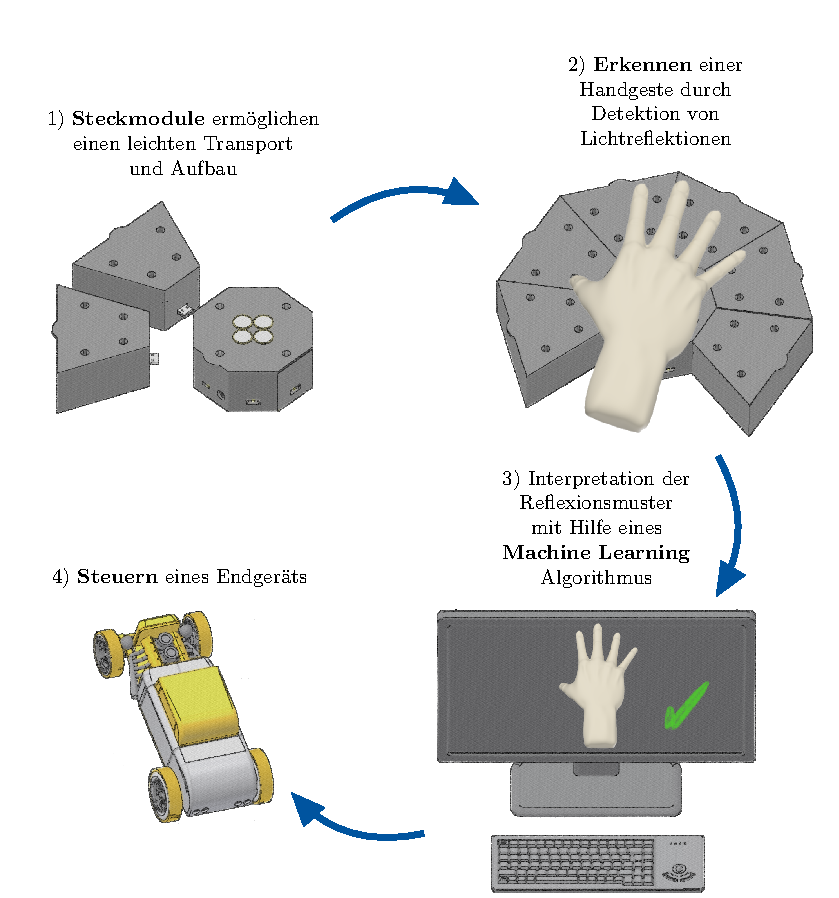
\includegraphics[scale=1.3]{../figures/tikz/GestikulaserAblauf.pdf}
	\caption{Schematische Darstellung der Funktionsweise des Gestikulasers.}
	\label{fig:FunktionsweiseGestikulaser}
\end{figure}

% -----------------------------------------------------%

\section{Die Beta-Version}

\begin{itemize}
	\item Anordnung der Photodioden auf einer Pressspanplatte in einem festgelegten Muster
	\item Arduino Uno zur Auswertung der Sensordaten
	\item Maximal 16 Photodioden anschließbar
\end{itemize}

\begin{figure}[h]
	\centering
	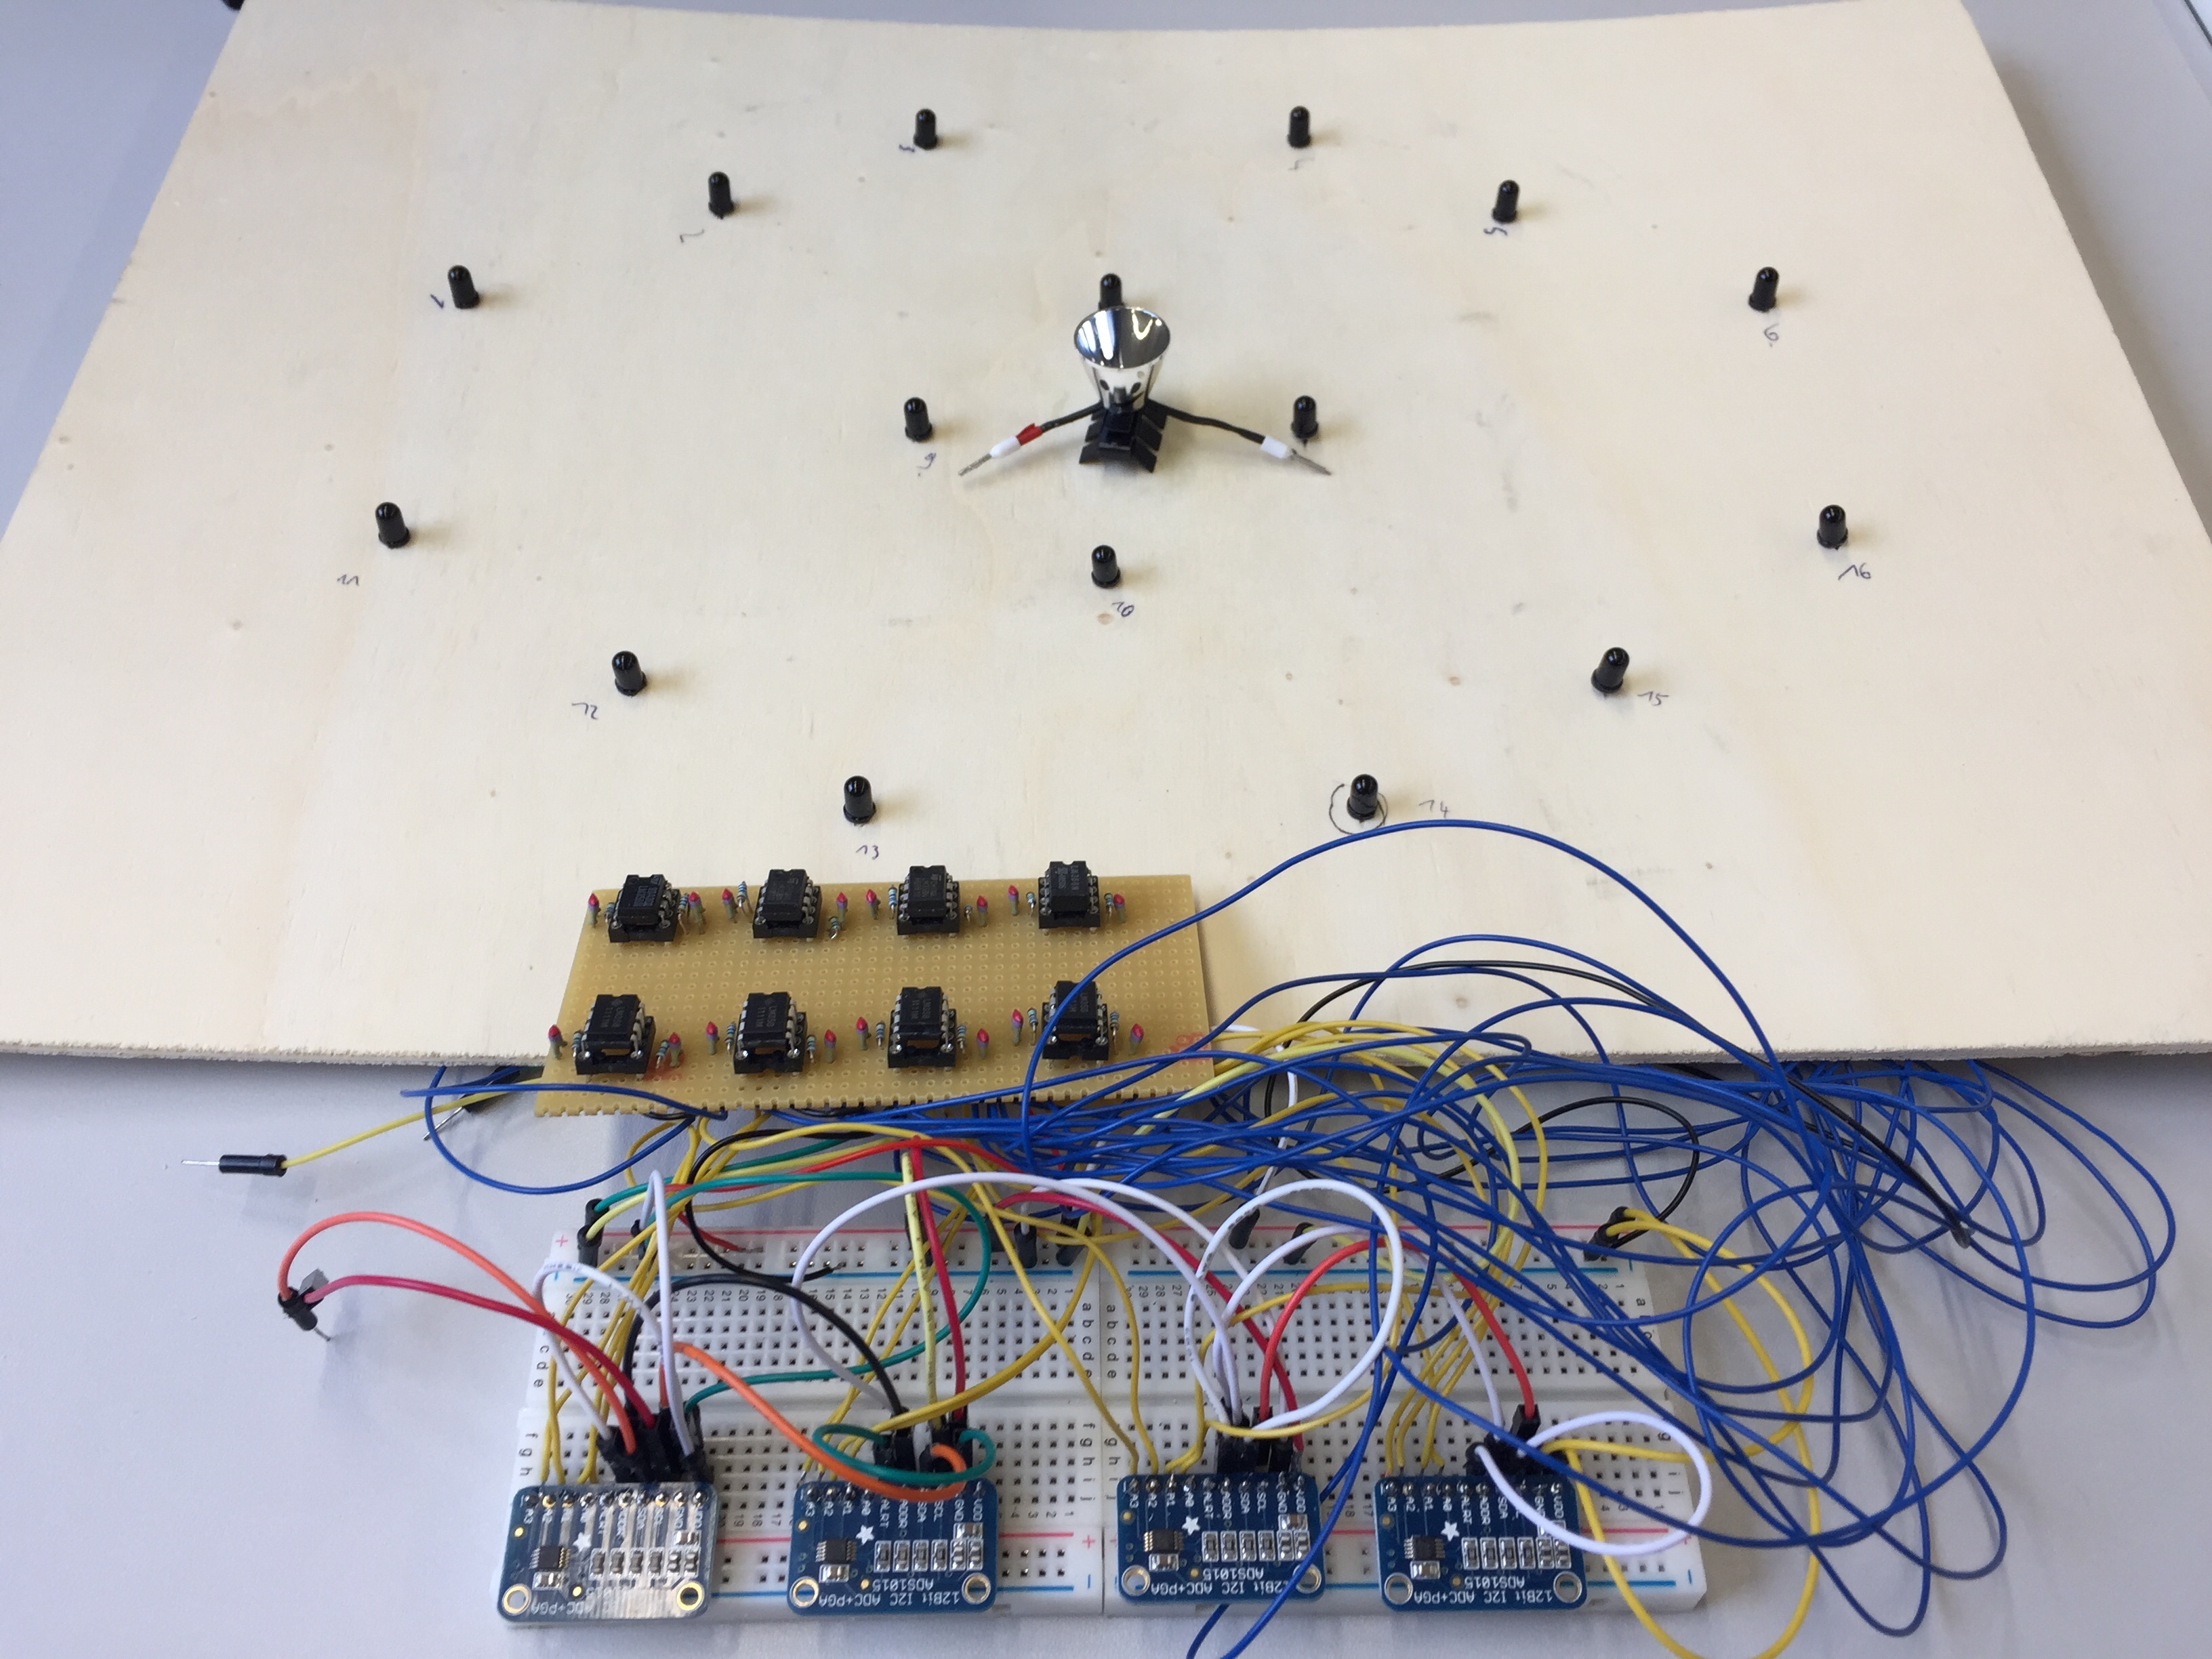
\includegraphics[scale=0.175]{../figures/PhotoplatteBeta.jpeg}
	\caption{Die Beta-Version der Photoplatte: Die Elektronik ist auf einer Steckplatine untergebracht, die Photodioden sind fest in der Platte verbaut.}
	\label{fig:PhotoplatteBeta}
\end{figure}

% -----------------------------------------------------%

\section{Photoplatte}
\noindent
Nachdem unsere Idee funktionierte, wollten wir nun unseren Gestikulaser modularer gestalten. Eine aus verschiedenen Steckmodulen zusammensetzbare Photoplatte sollte nun helfen, dieses Ziel zu erreichen.

\begin{itemize}
	\item Modulares Stecksystem aus insgesamt acht Komponenten
	\item Zentral gelegene, fest verbaute Lichtquelle
	\item Variable Anordnung der Photodioden
	\item Erweiterbar auf bis zu 128 Photodioden
\end{itemize}

\begin{figure}[h]
	\centering
	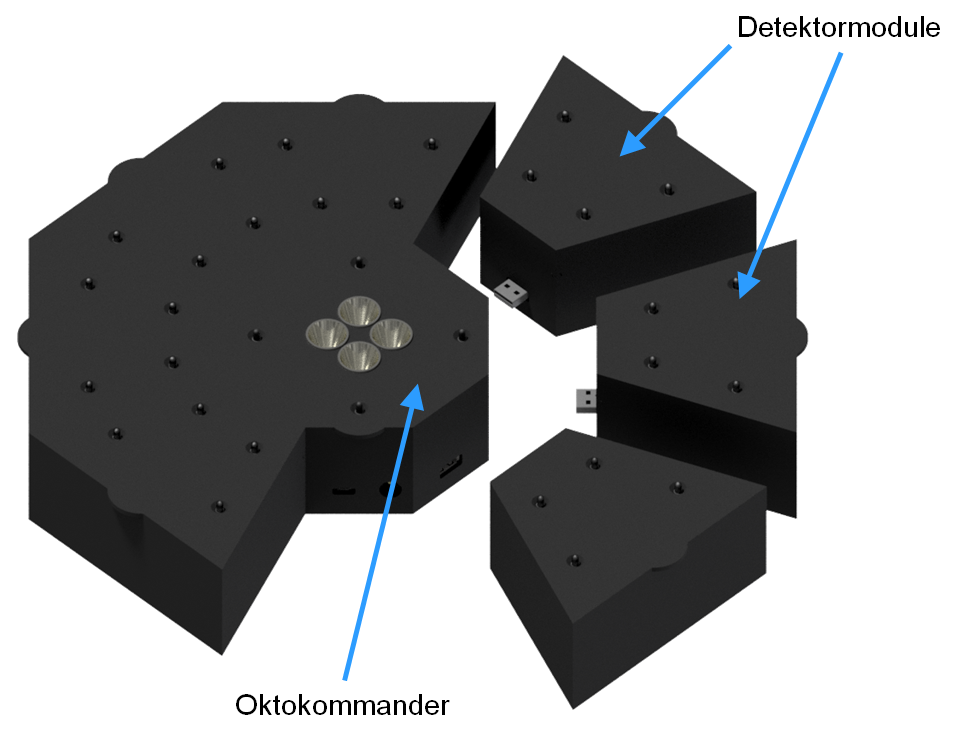
\includegraphics[scale=1.2]{../CAD_Bilder/Gestikulaser/Gestikulaser_beschriftet.png}
	\caption{Die neue modulare Photoplatte setzt sich aus einem Oktokommander und bis zu sieben Detektormodulen zusammen.}
	\label{fig:PhotoplatteAlpha}
\end{figure}

% -----------------------------------------------------%

\section{Oktokommander}
\noindent
Der Oktokommander ist das Steuersystem der gesamten Photoplatte.

\begin{figure}[h]
	\centering
	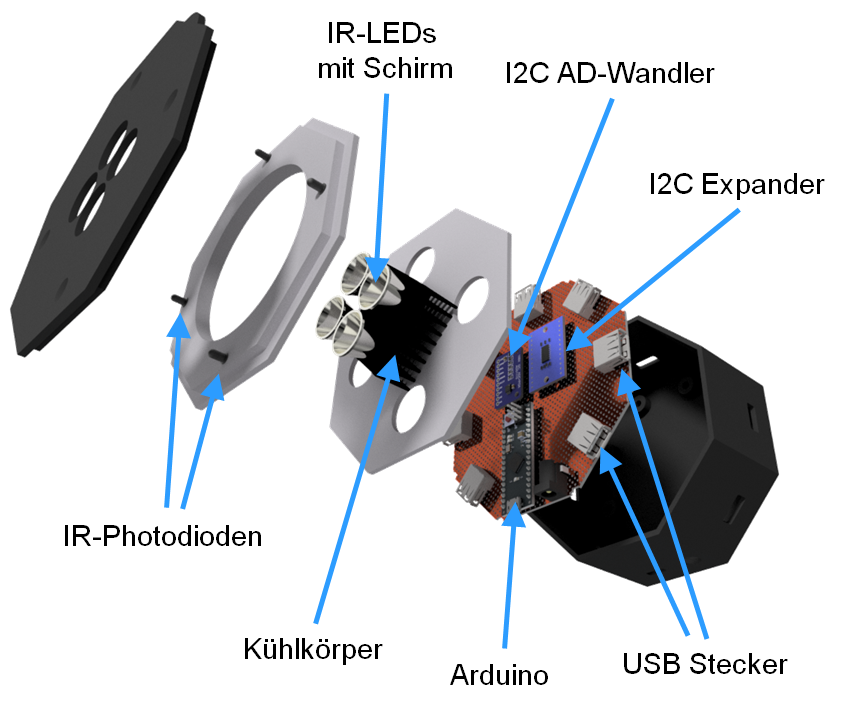
\includegraphics[scale=1.2]{../CAD_Bilder/Oktokommander/Oktokommander_beschriftet.png}
	\caption{Explosionsdarstellung des Oktokommanders.}
	\label{fig:Oktokommander}
\end{figure}

% -----------------------------------------------------%

\section{Detektormodul}
\noindent
Die Detektormodule sollen die Lichtreflexionen der Hand detektieren.

\begin{figure}[h]
	\centering
	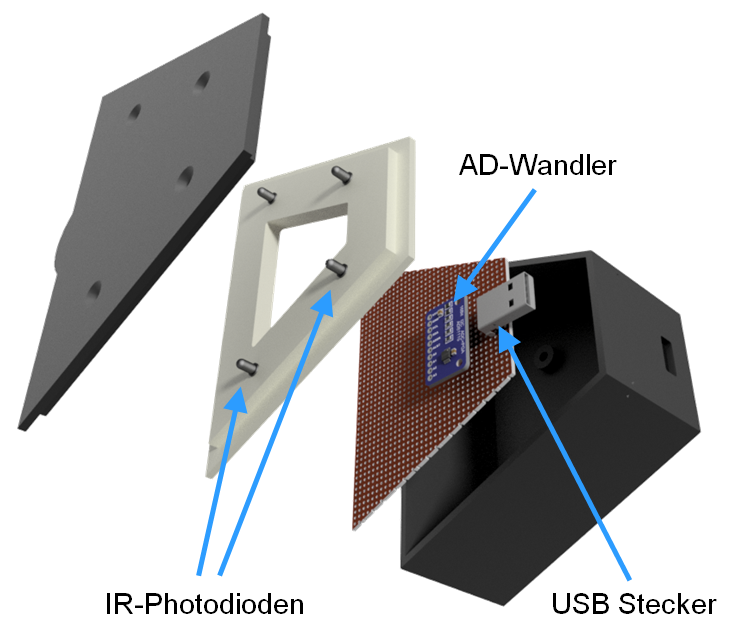
\includegraphics[scale=1.2]{../CAD_Bilder/Detektormodul/Detektormodul_beschriftet.png}
	\caption{Explosionsdarstellung eines Detektormoduls.}
	\label{fig:Detektormodul}
\end{figure}

% -----------------------------------------------------%

\section{Software}
\noindent
Die Kommunikation zwischen dem Mikrocontroller und dem Computer erfolgt über \texttt{Python} Skripte. Für die Erstellung des neuronalen Netzes wurde \texttt{TensorFlow}\texttrademark verwendet.

\centering

\vfill

\textbf{Trainingsphase}\\
\vspace{1.0cm}
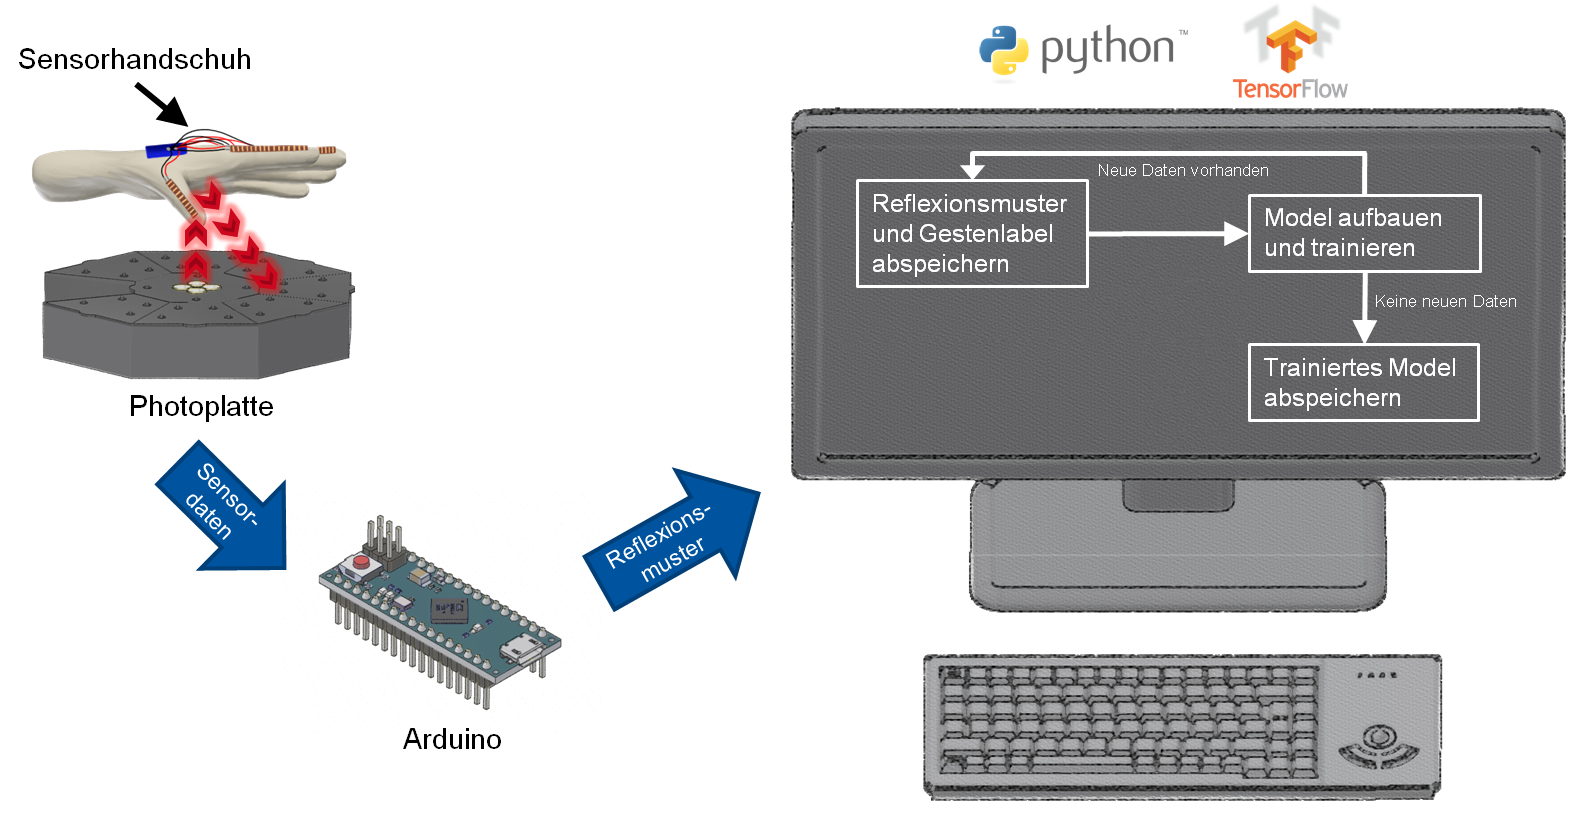
\includegraphics[scale=0.7]{../figures/Anlernphase.png}

\vfill

\textbf{Live-Betrieb}\\
\vspace{1.0cm}
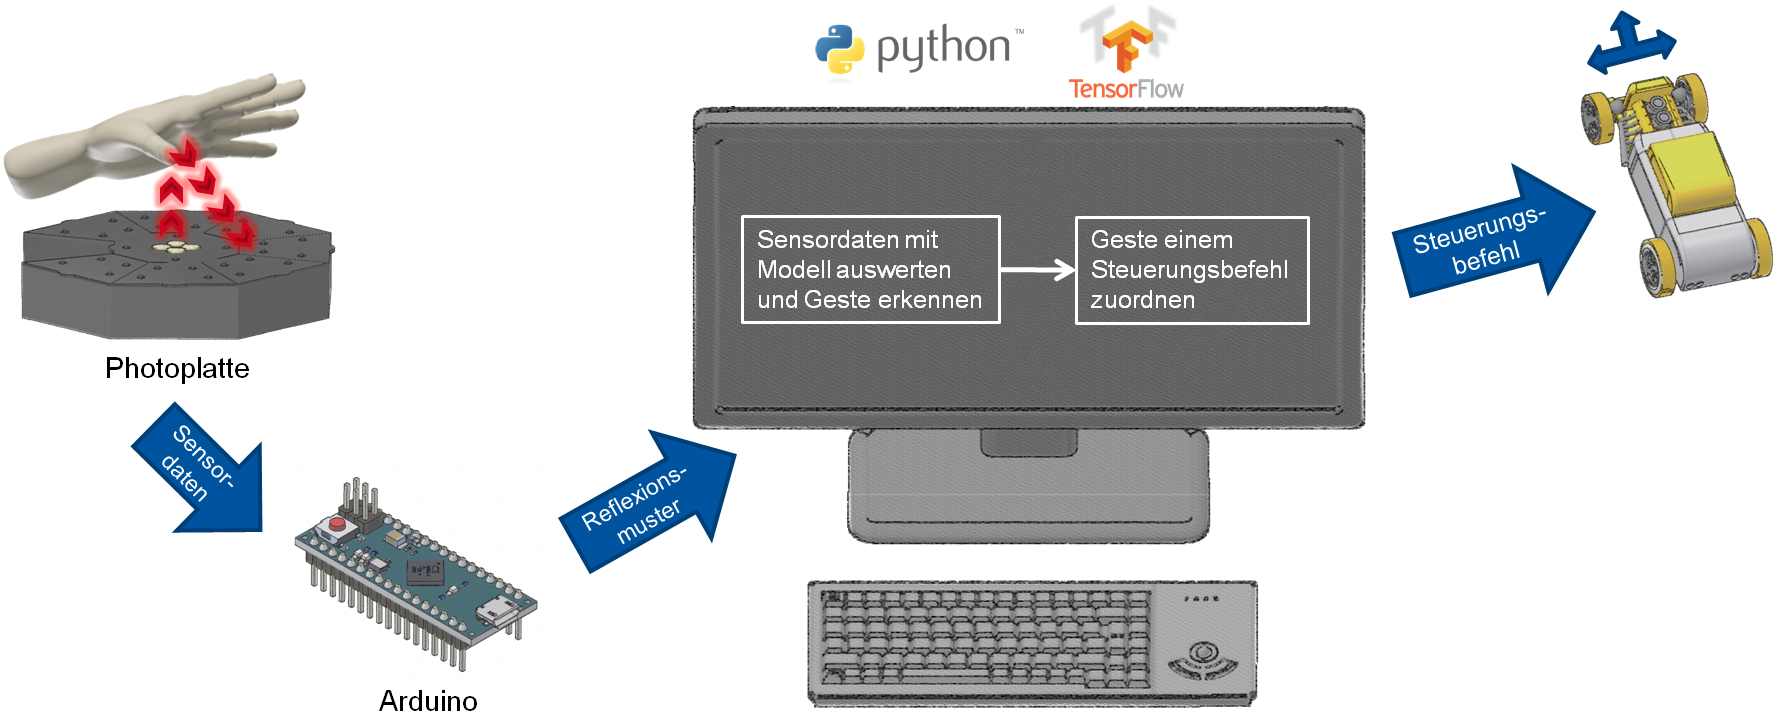
\includegraphics[scale=0.7]{../figures/LiveBetrieb.png}


% -----------------------------------------------------%

\section{Ausblick}
\noindent

\begin{itemize}
	\item Erkennung feinerer Gesten durch Berücksichtigung der Krümmung der einzelnen Finger
	\item Erweiterung auf dynamische Gesten
	\item Erhöhung des Abstands durch mehr Lichtleistung
\end{itemize}

\begin{figure}[h]
	\centering
	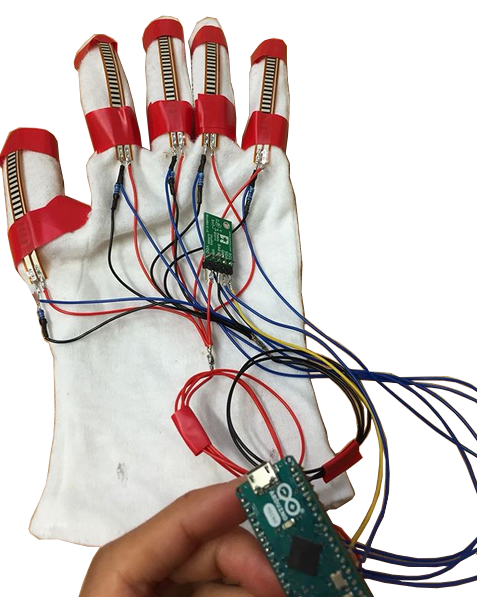
\includegraphics[scale=1.2]{../figures/Sensorhandschuh_transparent}
	\caption{Aktueller Prototyp eines Sensorhandschuhs. Es sind Biegesensoren für alle Finger, ein Gyroskop und ein Beschleunigungssensor im Einsatz. Die Sensordaten werden von einem Arduino Micro verarbeitet.}
	\label{fig:Sensorhandschuh}
\end{figure}

% -----------------------------------------------------%

\section{Sponsoren}
\noindent
Ein besonderen Dank gilt unseren Sponsoren: \\

\vfill

\begin{tabularx}{\textwidth}{L{10cm} c}
	Aconity3D GmbH & \noindent\parbox[c]{\hsize}{
\includegraphics[height=3cm]{../Logos/AC3D_Logo_Print-for-white.eps}} \\
	& \\
	Fraunhofer ILT & \noindent\parbox[c]{\hsize}{
\includegraphics[height=3cm]{../Logos/Fraunhofer_ILT_klein.png}} \\
	& \\
	Würth Electronik \quad \quad GmbH Co. KG & \noindent\parbox[c]{\hsize}{
\includegraphics[height=3cm]{../Logos/Wuerth.png}}
\end{tabularx} \\

\end{multicols}

\conference{
	\raisebox{0.5cm}[0cm]{
\includegraphics[height=3cm]{../Logos/VDE.png} } \hfill
	\raisebox{1.25cm}[0cm]{
\includegraphics[height=1.5cm]{../Logos/Faulhaber.png}} \hfill
	\raisebox{0cm}[0cm]{
\includegraphics[height=4cm]{../Logos/micronit.png}} \hfill
	\raisebox{0cm}[0cm]{
\includegraphics[height=4cm]{../Logos/electronica.png}} \hfill 
	\raisebox{0cm}[0cm]{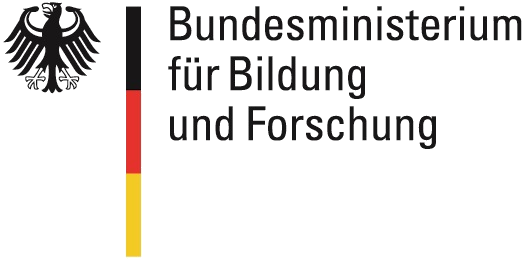
\includegraphics[height=4cm]{../Logos/BMBF.png}}
}

\end{document}